%%%%%%%%%%%%%%%%%%%%%%%%%%%%%%%%%%%%%%%%%%%%%%%%%%%%%%%%%%%%%%%%%%%%%%%%%%%%%%%%%
%% Documenclass 
%%%%%%%%%%%%%%%%%%%%%%%%%%%%%%%%%%%%%%%%%%%%%%%%%%%%%%%%%%%%%%%%%%%%%%%%%%%%%%%%%
\documentclass[a4paper,oneside,titlepage]{report}
%%%%%%%%%%%%%%%%%%%%%%%%%%%%%%%%%%%%%%%%%%%%%%%%%%%%%%%%%%%%%%%%%%%%%%%%%%%%%%%%%
%% Packages
%%%%%%%%%%%%%%%%%%%%%%%%%%%%%%%%%%%%%%%%%%%%%%%%%%%%%%%%%%%%%%%%%%%%%%%%%%%%%%%%%
\usepackage[english]{babel}
\usepackage{amsmath}
\usepackage{complexity}
\usepackage[T1]{fontenc}
\usepackage[utf8]{inputenc}
\usepackage[pdftex]{graphicx} %%Graphics in pdfLaTeX
\usepackage{a4wide} %%Smaller margins, more text per page.
\usepackage{longtable} %%For tables that exceed a page width
\usepackage{pdflscape} %%Adds PDF support to the landscape environment of package
\usepackage{caption} %%Provides many ways to customise the captions in floating environments like figure and table
\usepackage{float} %%Improves the interface for defining floating objects such as figures and tables
\usepackage[tablegrid,nochapter]{vhistory} %%Vhistory simplifies the creation of a history of versions of a document
\usepackage[nottoc]{tocbibind} %%Automatically adds the bibliography and/or the index and/or the contents, etc., to the Table of Contents listing
\usepackage[toc,page]{appendix} %%The appendix package provides various ways of formatting the titles of appendices
\usepackage{pdfpages} %%This package simplifies the inclusion of external multi-page PDF documents in LATEX documents
\usepackage[rightcaption]{sidecap} %%Defines environments called SCfigure and SCtable (analogous to figure and table) to typeset captions sideways
\usepackage{cite} %%The package supports compressed, sorted lists of numerical citations, and also deals with various punctuation and other issues of representation, including comprehensive management of break points
\usepackage[]{acronym} %%This package ensures that all acronyms used in the text are spelled out in full at least once. It also provides an environment to build a list of acronyms used
\usepackage[pdftex,scale={.8,.8}]{geometry} %%The package provides an easy and flexible user interface to customize page layout, implementing auto-centering and auto-balancing mechanisms so that the users have only to give the least description for the page layout. For example, if you want to set each margin 2cm without header space, what you need is just \usepackage[margin=2cm,nohead]{geometry}.
\usepackage{layout} %%The package defines a command \layout, which will show a summary of the layout of the current document
\usepackage{subfigure} %%Provides support for the manipulation and reference of small or ‘sub’ figures and tables within a single figure or table environment.
\usepackage[toc]{glossaries} %%The glossaries package supports acronyms and multiple glossaries, and has provision for operation in several languages (using the facilities of either babel or polyglossia).
\usepackage[left,pagewise,modulo]{lineno} %%Adds line numbers to selected paragraphs with reference possible through the LATEX \ref and \pageref cross reference mechanism
\usepackage[pdftex,colorlinks=false,hidelinks,pdfstartview=FitV]{hyperref}%%The hyperref package is used to handle cross-referencing commands in LATEX to produce hypertext links in the document. 
\usepackage{metainfo}
\usepackage[pagestyles,raggedright]{titlesec}
\usepackage{etoolbox}
\usepackage{%
	array, %%An extended implementation of the array and tabular environments which extends the options for column formats, and provides "programmable" format specifications
	booktabs, %%The package enhances the quality of tables in LATEX, providing extra commands as well as behind-the-scenes optimisation
	dcolumn, %%
	rotating,
	shortvrb,
	units,
	url,
	lastpage,
	longtable,
	lscape,
	qtree,
	skmath,	
}
%%%%%%%%%%%%%%%%%%%%%%%%%%%%%%%%%%%%%%%%%%%%%%%%%%%%%%%%%%%%%%%%%%%%%%%%%%%%%%%%%
%% Java --> latex 
%%%%%%%%%%%%%%%%%%%%%%%%%%%%%%%%%%%%%%%%%%%%%%%%%%%%%%%%%%%%%%%%%%%%%%%%%%%%%%%%%
\usepackage{listings}
\usepackage{color}
\definecolor{pblue}{rgb}{0.13,0.13,1}
\definecolor{pgreen}{rgb}{0,0.5,0}
\definecolor{pred}{rgb}{0.9,0,0}
\definecolor{pgrey}{rgb}{0.46,0.45,0.48}
\usepackage{inconsolata}
%%Listing style for java.
\definecolor{dkgreen}{rgb}{0,0.6,0}
\definecolor{gray}{rgb}{0.5,0.5,0.5}
\definecolor{mauve}{rgb}{0.58,0,0.82}
\lstset{frame=tb,
	language=Java,
	aboveskip=3mm,
	belowskip=3mm,
	showstringspaces=false,
	columns=flexible,
	basicstyle={\small\ttfamily},
	numbers=left,
	numberstyle=\tiny\color{gray},
	keywordstyle=\color{blue},
	commentstyle=\color{dkgreen},
	stringstyle=\color{mauve},
	breaklines=true,
	breakatwhitespace=true,
	tabsize=3
}

%%%%%%%%%%%%%%%%%%%%%%%%%%%%%%%%%%%%%%%%%%%%%%%%%%%%%%%%%%%%%%%%%%%%%%%%%%%%%%%%%
\setlength{\parindent}{0pt}
\setlength{\parskip}{.5\baselineskip}
%%%%%%%%%%%%%%%%%%%%%%%%%%%%%%%%%%%%%%%%%%%%%%%%%%%%%%%%%%%%%%%%%%%%%%%%%%%%%%%%%
%% Inserting the metadata
%%%%%%%%%%%%%%%%%%%%%%%%%%%%%%%%%%%%%%%%%%%%%%%%%%%%%%%%%%%%%%%%%%%%%%%%%%%%%%%%%

\def\Company{\textit{MJZSoft Ltd.}}
\def\Institute{\textit{Fontys Hogeschool Techniek en Logistiek, Venlo}}
\def\Authors{Prepared by Mahdi J. Ansari }

\def\BoldTitle{Software Requirements Specification}
\def\Subtitle{for \\ \textit{iBrief} \\}


\title{\textbf{\BoldTitle}\\\Subtitle}
\author{\Authors \\ at \Company\\}
\date{Calgary, October 08, 2023}

%%%%%%%%%%%%%%%%%%%%%%%%%%%%%%%%%%%%%%%%%%%%%%%%%%%%%%%%%%%%%%%%%%%%%%%%%%%%%%%%%
%% Creation of pdf information
%%%%%%%%%%%%%%%%%%%%%%%%%%%%%%%%%%%%%%%%%%%%%%%%%%%%%%%%%%%%%%%%%%%%%%%%%%%%%%%%%
\hypersetup{pdfinfo={
		Title={Title},
		Author={TR},
		Subject={Report}
	}}
%%%%%%%%%%%%%%%%%%%%%%%%%%%%%%%%%%%%%%%%%%%%%%%%%%%%%%%%%%%%%%%%%%%%%%%%%%%%%%%%%
%% Creating the frontpage
%%%%%%%%%%%%%%%%%%%%%%%%%%%%%%%%%%%%%%%%%%%%%%%%%%%%%%%%%%%%%%%%%%%%%%%%%%%%%%%%%
\AtBeginDocument{
	\maketitle
	\thispagestyle{empty}
}
%%%%%%%%%%%%%%%%%%%%%%%%%%%%%%%%%%%%%%%%%%%%%%%%%%%%%%%%%%%%%%%%%%%%%%%%%%%%%%%%%
%% Creation of the header
%%%%%%%%%%%%%%%%%%%%%%%%%%%%%%%%%%%%%%%%%%%%%%%%%%%%%%%%%%%%%%%%%%%%%%%%%%%%%%%%%
\patchcmd{\chapter}{plain}{short}{}{} %$ <-- the header on chapter 1
%%%%%%%%%%%%%%%%%%%%%%%%%%%%%%%%%%%%%%%%%%%%%%%%%%%%%%%%%%%%%%%%%%%%%%%%%%%%%%%%%
%% Creation of page-styles
%%%%%%%%%%%%%%%%%%%%%%%%%%%%%%%%%%%%%%%%%%%%%%%%%%%%%%%%%%%%%%%%%%%%%%%%%%%%%%%%%
\newpagestyle{long}{%
	\sethead[\thepage][][\chaptername\ \thechapter:\ \chaptertitle]{\chaptername\ \thechapter:\ \chaptertitle}{}{\thepage}
	\headrule
}
\newpagestyle{short}{%
	\sethead[\thepage][][]{}{}{\thepage}
	\headrule
}
%%%%%%%%%%%%%%%%%%%%%%%%%%%%%%%%%%%%%%%%%%%%%%%%%%%%%%%%%%%%%%%%%%%%%%%%%%%%%%%%%
%% Include the glossary entries from the separate file
%%%%%%%%%%%%%%%%%%%%%%%%%%%%%%%%%%%%%%%%%%%%%%%%%%%%%%%%%%%%%%%%%%%%%%%%%%%%%%%%%
\newglossaryentry{iOS}{
  name={iOS},
  description={Apple's mobile operating system used for its iPhone, iPad, and iPod Touch devices.}
}

\newglossaryentry{Android}{
  name={Android},
  description={An open-source mobile operating system developed by Google.}
}

\newglossaryentry{React}{
  name={React},
  description={A JavaScript library for building user interfaces, maintained by Facebook.}
}

\newglossaryentry{AWS}{
  name={AWS},
  description={Amazon Web Services, a subsidiary of Amazon providing cloud computing platforms and APIs.}
}

\newglossaryentry{client application}{
  name={client application},
  description={A software application that runs on the client side, typically on a user's device, and connects to a server to fetch or send data.}
}

\newglossaryentry{dashboard application}{
  name={dashboard application},
  description={An application interface that provides users with an overview and control of specific metrics or features.}
}

\newglossaryentry{back-end}{
  name={back-end},
  description={The server-side of an application, responsible for data storage, retrieval, and processing.}
}

\newglossaryentry{UI}{
  name={UI},
  description={User Interface, the space where user interactions occur with a digital product or service.}
}
\renewcommand*{\glossarysection}[2][]{\relax}% Suppress the Glossary header
\makeglossaries
%%%%%%%%%%%%%%%%%%%%%%%%%%%%%%%%%%%%%%%%%%%%%%%%%%%%%%%%%%%%%%%%%%%%%%%%%%%%%%%%%
%% DOCUMENT
%%%%%%%%%%%%%%%%%%%%%%%%%%%%%%%%%%%%%%%%%%%%%%%%%%%%%%%%%%%%%%%%%%%%%%%%%%%%%%%%%
\begin{document}
\pagenumbering{roman}
\DeclareGraphicsExtensions{.pdf,.jpg,.png}
\pagestyle{short}
\newpage
%%%%%%%%%%%%%%%%%%%%%%%%%%%%%%%%%%%%%%%%%%%%%%%%%%%%%%%%%%%%%%%%%%%%%%%%%%%%%%%%%
%% Table of contents
%%%%%%%%%%%%%%%%%%%%%%%%%%%%%%%%%%%%%%%%%%%%%%%%%%%%%%%%%%%%%%%%%%%%%%%%%%%%%%%%%
\tableofcontents % Inhaltsverzeichnis
\pagestyle{long}
%%%%%%%%%%%%%%%%%%%%%%%%%%%%%%%%%%%%%%%%%%%%%%%%%%%%%%%%%%%%%%%%%%%%%%%%%%%%%%%%%
%% Version table insertion
%%%%%%%%%%%%%%%%%%%%%%%%%%%%%%%%%%%%%%%%%%%%%%%%%%%%%%%%%%%%%%%%%%%%%%%%%%%%%%%%%
\chapter*{Revision History}
\addcontentsline{toc}{chapter}{Revision History}
\begin{versionhistory}
	\vhEntry{1.0}{10.10.2023}{Mahdi J. Ansari}{Made the structure of the document}


\end{versionhistory}
\pagenumbering{arabic}
%%%%%%%%%%%%%%%%%%%%%%%%%%%%%%%%%%%%%%%%%%%%%%%%%%%%%%%%%%%%%%%%%%%%%%%%%%%%%%%%%
%% Inserting all the content
%%%%%%%%%%%%%%%%%%%%%%%%%%%%%%%%%%%%%%%%%%%%%%%%%%%%%%%%%%%%%%%%%%%%%%%%%%%%%%%%%
    \chapter{Introduction}\label{ch:Introduction}
        \section{Purpose}
            This document serves as a comprehensive guide to the functional and non-functional requirements of the \textbf{iBrief} application. It provides a detailed overview of the key features, behaviors, and interfaces to be implemented in its inaugural release.

\subsection{Objective}
    The primary objective of this document is to offer a structured and lucid insight into the \textbf{iBrief} application's requirements. Specifically, it aims to:
        \begin{itemize}
            \item Define the core functionalities, behaviors, and expectations of the application.
            \item Establish a consistent foundation for development, design, and testing activities.
            \item Serve as an authoritative reference for all project stakeholders, ensuring alignment in understanding and expectations.
            \item Detail the user interface (\gls{UI}) design and workflow for the \gls{mobile application}s.
            \item Guarantee alignment with overarching project objectives and user requirements.
        \end{itemize}

\subsection{Scope}
    This document encompasses both the functional and non-functional aspects of the \textbf{iBrief} application. It emphasizes the features and behaviors that are central to its primary functionality and provides a road-map for its development trajectory, covering the initial release and setting the stage for subsequent enhancements.

    By meticulously documenting the functional requirements, non-functional constraints, and \gls{UI} expectations, this document ensures a shared understanding of the \textbf{iBrief} application's mission and capabilities among all project participants. It remains a crucial touchstone throughout the development life-cycle, aiding in the successful realization and launch of the \textbf{iBrief} application.






        \section{Document Conventions}
            \subsection{Terminology}
Throughout this requirement document, specific terminology and conventions are utilized to ensure clarity and emphasis:
    \begin{itemize}
        \item \textbf{Term in Bold:} Important project-related terms, concepts, or headings, such as "\textbf{iBrief}" or "\textbf{Product Scope}," are highlighted using bold.
        
        \item \textit{Italicized Term:} Italics emphasize specific terms, or indicate variables or placeholders, like \textit{user stories} or \textit{deliverable}.
        
        \item \texttt{Monospaced Text:} Technical elements, including \texttt{code snippets} or \texttt{file paths}, are represented using a monospaced font.
        
        \item \text{[Square Brackets]}: Square brackets indicate placeholders, e.g., [Project Sponsor's Name] or [Date], to be replaced with contextually relevant information.
    \end{itemize}

\subsection{Abbreviations and Acronyms}
For conciseness and clarity, this document incorporates abbreviations and acronyms. A comprehensive list of these can be found in appendix \ref{apn:glossary}.

\subsection{Formatting Conventions}
This document adheres to the following formatting conventions for consistency and enhanced readability:

    \begin{itemize}
        \item \textbf{Section Headings:} Headings are numbered and presented in title case, facilitating quick navigation and reference.
        
        \item \textit{Italicized Text:} Italics are reserved for emphasis, variable names, and placeholders.
        
        \item \texttt{Monospaced Font:} Code snippets, \gls{URL}s, file paths, and other technical references employ a monospaced font.
        
        \item Bullet Points and Enumerations: Lists use bullet points, while sequential or numbered lists employ enumerations.
        
        \item \textbf{Hyperlinks:} External resources or web addresses are represented as hyperlinks, typically colored and underlined.
    \end{itemize}

\subsection{References and Citations}
All external references, be it to documents, standards, or other resources, are cited in alignment with recognized citation styles like IEEE, APA, or a designated company standard.

\subsection{Version Control}
Version control is in place for this document, ensuring accurate tracking of changes and revisions. The document's revision history provides a detailed record of edits over time.

\subsection{Review and Approval}
Key stakeholders, including the project sponsor and project manager, review and approve this requirements document. This process guarantees alignment with the overarching project vision and objectives.

        \section{Intended Audience and Reading Suggestions}
            \subsection{Intended Audience}
This requirements document is crafted for a diverse set of stakeholders, both technical and non-technical. The intended audiences include:

    \begin{itemize}
        \item \textbf{Development Team:} Software developers and programmers tasked with realizing the application's functionalities based on the specifications provided.
        
        \item \textbf{Design Team:} \gls{UI} and \gls{UX} designers shaping the visual layout and ensuring optimal user interaction with the application.
        
        \item \textbf{Testing Team:} \gls{QA} professionals validating the application's conformity to its functional requirements and ensuring robustness.
        
        \item \textbf{Project Management:} Overseeing the project's progression, timelines, and resource allocation.
        
        \item \textbf{Stakeholders:} Including project sponsors, investors, system architects, local authorities, government agencies, and \gls{end-user}s such as citizens.
        
        \item \textbf{Documentation Team:} Drafting user manuals, help guides, and other relevant documentation using this document as a primary reference.
    \end{itemize}

This document offers insights tailored to each audience. Technical teams will find detailed specifications, while non-technical stakeholders can grasp the overarching project vision and objectives.

\subsection{Reading Suggestions}
For a structured navigation through this document, we suggest the following approach:

    \begin{itemize}
        \item \textbf{Project Overview:} Begin with the "Project Description" for a holistic understanding of the \textbf{iBrief} application's vision.
        
        \item \textbf{Product Scope:} Delve deeper into the "Product Scope" for insights on the application's functionalities, objectives, and key deliverables.
        
        \item \textbf{Stakeholder Perspective:} The "Stakeholders" section elucidates the primary entities associated with the project and their roles.
        
        \item \textbf{Technical Details:} Technical members should explore the technical specifics in the "Product Scope" and other relevant sections.
        
        \item \textbf{Dependencies and Risks:} The "Dependencies" and "Risks" sections shed light on potential challenges and interdependencies.
        
        \item \textbf{Change Control and Approval:} Familiarize yourself with the modus operandi for managing project changes in the "Change Control" section, wrapping up with the "Approval" section.
        
        \item \textbf{Appendices and Additional Resources:} Supplement your understanding by referring to appendices and any provided additional resources.
    \end{itemize}
    
Active engagement, discussions, and seeking clarifications are encouraged to ensure all stakeholders share a unified understanding of the project's scope and aspirations.

        \section{Product Scope}
            \subsection{Project Overview and Description}
    The \textbf{iBrief} application serves as an integrated digital platform, empowering citizens to promptly report urban issues to local authorities. Aimed at enhancing public infrastructure management and community welfare, this initiative simplifies the reporting, tracking, and resolution processes. Although the application's current moniker is `iBrief', potential rebranding and white labeling might occur for marketing strategies. 

\subsection{Objectives and Features}
    The \textbf{iBrief} application's core objectives encompass:
    \begin{enumerate}[label=\alph*)]
        \item Offering an intuitive mobile platform for incident reporting.
        \item Ensuring traceability from issue submission to resolution.
        \item Facilitating seamless communication between citizens and local authorities.
        \item Augmenting urban safety, cleanliness, and overall living standards.
        \item Widening accessibility across iOS and Android users.
    \end{enumerate}

    To realize these objectives, \textbf{iBrief} will incorporate:
    \begin{itemize}
        \item User-centric account management.
        \item Simplified issue reporting with \gls{GPS} location tagging.
        \item Support for multimedia attachments.
        \item Real-time issue tracking and notifications.
        \item Integration with local authority systems.
        \item A comprehensive \gls{web-based} administrative dashboard.
    \end{itemize}

\subsection{Deliverables and Scope}
    The key project deliverables include:
    \begin{enumerate}
        \item A \gls{iOS} \gls{client application}.
        \item A robust \gls{Android} counterpart.
        \item A \gls{React}-powered administrative dashboard.
        \item A secure, \gls{AWS}-hosted back-end infrastructure.
    \end{enumerate}
    
    The project's ambit covers the creation and deployment of mobile applications, the \gls{web-based} dashboard, and the foundational back-end. This also entails the system's integration with existing local authority infrastructures for issue resolution efficacy.
    
\subsection{Stakeholders and Dependencies}
    Key project \gls{stakeholders} comprise:
    \begin{itemize}
        \item End-users or citizens.
        \item Local governing bodies.
        \item Project overseers and sponsors.
        \item Development and \gls{QA} personnel.
    \end{itemize}
    
    The project hinges on:
    \begin{itemize}
        \item Gaining access to local authority data and systems.
        \item Ensuring stakeholder collaboration and approvals.
        \item Procuring necessary development and testing resources.
    \end{itemize}

\subsection{Assumptions, Risks, and Change Management}
    The project's foundational assumptions include:
    \begin{itemize}
        \item Users possessing internet-enabled smartphones.
        \item Collaborative disposition of local authorities.
        \item Adequate resource allocation.
    \end{itemize}

    Foreseen project risks encompass:
    \begin{itemize}
        \item System integration hurdles.
        \item Varied user engagement levels.
        \item Data privacy and security challenges.
        \item Potential technical roadblocks.
    \end{itemize}
    
    A structured change control process will be in place, mandating documented changes to undergo impact assessments and secure approvals from key \gls{stakeholders} before execution.

        \section{User Characteristics (Roles)}
            This section delineates the varied user personas that will interface with the \textbf{iBrief} application. It outlines their primary responsibilities and interactions with the system.

\begin{itemize}
    \item \textbf{End-Users (Citizens)}: These are general users concerned about urban aspects and public infrastructure. They utilize mobile devices to report issues and may appreciate incentives for their efforts. Their primary interactions involve:
        \begin{itemize}
            \item Reporting city-related issues.
            \item Tracking the status of their reports.
        \end{itemize}

        Figure \ref{fig:user-is-using-the-app} shows steps that a user follows for reporting an issue.
        \newpage
        \begin{figure}[!ht]
            \centering
            \caption{User is using the application}
            \label{fig:user-is-using-the-app}
            \begin{minipage}{0.4\textwidth}
                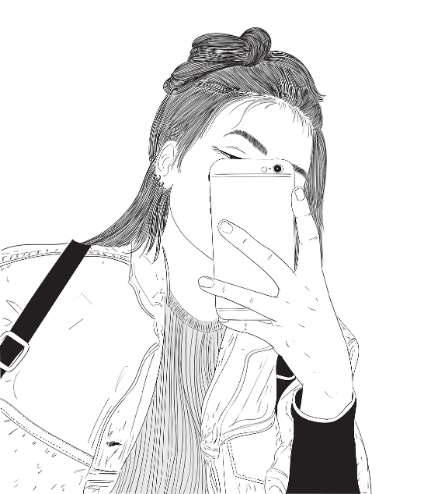
\includegraphics[width=\linewidth]{images/Image_ (1).png} 
            \end{minipage}%
            \hspace{0.05\textwidth} % Space between the image and the text
            \begin{minipage}{0.5\textwidth}
                I like to use my smartphone to take a picture and report this issue!
                \begin{enumerate}
                    \raggedright
                    \item Just open the app.
                    \item Make a new report.
                    \item Add address or use Geo location information.
                    \item If the city does not supported you will be informed, otherwise:
                    \item Select a category.
                    \item Add multimedia (i.e., picture, video, voice).
                    \item Press on submit button.
                    \item You will be updated regarding the progress.
                \end{enumerate}
            \end{minipage}
        \end{figure}

    \item \textbf{Officers (Local Authorities)}: Officers oversee all reported issues, ensuring timely and efficient resolution. Their responsibilities encompass:
        \begin{itemize}
            \item Monitoring all reports.
            \item Exporting report data.
            \item Integrating workflows with other applications.
        \end{itemize}

    \item \textbf{Agents (Issue Resolvers)}: Agents are tasked with the on-ground resolution of reported issues. Their workflow includes:
        \begin{itemize}
            \item Visiting reported locations.
            \item Updating the report's status throughout the resolution process.
        \end{itemize}

    \item \textbf{Administrators (Customer Point of Contacts)}: Administrators hold the highest permissions within their organization, acting as liaisons between the local authority and the \textbf{iBrief} team. They are accountable for:
        \begin{itemize}
            \item Contract management.
            \item Granting permissions.
            \item Configuring application workflows.
        \end{itemize}

    \item \textbf{Support Team}: Supports assist both the end-users and officers in using the application. They can:
        \begin{itemize}
            \item Address application-related queries.
            \item Escalate technical issues to developers.
        \end{itemize}

    \item \textbf{Sales Team}: Holding superior permissions than the support team, the sales team's responsibilities include:
        \begin{itemize}
            \item Customer relationship management.
            \item Contract preparation.
            \item Account management.
        \end{itemize}

    \item \textbf{Super Users (Developers and QA Team)}: Possessing the apex level of permissions, super users can:
        \begin{itemize}
            \item Access all system features.
            \item Test and validate application functionalities.
            \item Toggle between various roles for testing purposes.
        \end{itemize}
\end{itemize}

    

    \chapter{Overall Description}\label{ch:Overall Description}
        \section{Product Perspective}   
            The \textbf{iBrief} application emerges as a self-contained \gls{mobile application} tailored for users' smartphones. While it operates autonomously, it leverages external web services and \gls{API}s, especially for location-based services and data archival. The central ethos of \textbf{iBrief} revolves around offering an intuitive platform for citizens to voice concerns and report city-centric issues, coupled with a robust \gls{back-end} system adept at issue orchestration and resolution.

\subsection{Benefits}

The inception of \textbf{iBrief} heralds a plethora of advantages for both its end-users and the overseeing city administrations:

    \begin{itemize}
        \item \textbf{Elevated Civic Participation:} \textbf{iBrief} stands as a catalyst, galvanizing citizens to immerse themselves in urban stewardship. By demystifying the issue-reporting process and championing active community involvement, \textbf{iBrief} sows the seeds for a cohesive and proactive urban community.
        
        \item \textbf{Swift Issue Redressal:} By instituting real-time tracking and systematic categorization, \textbf{iBrief} empowers city authorities to judiciously marshal resources. Such a methodical approach not only truncates resolution timelines but also amplifies user satisfaction by ensuring issues don't languish in administrative labyrinths.
        
        \item \textbf{Data-Driven Urban Governance:} \textbf{iBrief} is not just a reactive tool—it's a proactive informant. The data it amasses offers a granular view of urban challenges, allowing authorities to harness these insights for strategic decision-making, from resource allocation to infrastructural enhancements.
        
        \item \textbf{Transparent and Fluid Communication:} With \textbf{iBrief}, communication isn't an afterthought—it's integral. Users stay abreast with real-time updates on their concerns, instilling a sense of transparency. Concurrently, the seamless dialogue between citizens, support cadres, and authorities guarantees that resolutions aren't just efficient—they're collaborative.
    \end{itemize}

In essence, the \textbf{iBrief} ecosystem doesn't just address urban challenges—it anticipates them. By fostering civic engagement, hastening resolutions, leveraging data insights, and promoting transparent dialogues, \textbf{iBrief} is redefining urban living standards and enhancing the collective quality of life.

        \section{Product Functions}
            The \textbf{iBrief} application is more than just a reporting tool—it's a comprehensive platform that integrates various functionalities to elevate urban living. Here are the pivotal functions that define the \textbf{iBrief} experience:

\begin{itemize}
    \item \textbf{User Onboarding:} Streamlined user registration and login ensure a seamless entry into the \textbf{iBrief} ecosystem.
    
    \item \textbf{Intuitive Reporting:} Users can effortlessly report issues, enriched with textual descriptions, illustrative photos, and informative videos.
    
    \item \textbf{Precision in Reporting:} The integration of GPS-based location tagging ensures that issues are pinpointed with utmost accuracy, eliminating ambiguities in location reporting.
    
    \item \textbf{Dynamic Issue Tracking:} Stay updated with real-time tracking, which chronicles the journey of an issue from its report to its resolution.
    
    \item \textbf{Proactive Notifications:} Users aren't left in the dark—notifications offer timely updates about the progress and status of reported issues.
    
    \item \textbf{Seamless Integration:} \textbf{iBrief} doesn't operate in isolation—it synergizes with local authority systems to expedite and streamline issue resolutions.
    
    \item \textbf{Structured Workflow:} Issue resolvers (i.e., agents) are equipped with a clear workflow, ensuring that each step in the resolution process is systematic and efficient.
    
    \item \textbf{Tailored User Experience:} From personal account settings to user-specific data, \textbf{iBrief} offers customization at your fingertips.
    
    \item \textbf{Engagement Ecosystem:} Reporting isn't just a civic duty—it's rewarding. With incentives and rewards, \textbf{iBrief} fosters a proactive and involved user base.
    
    \item \textbf{Holistic Urban Platform:} \textbf{iBrief} goes beyond just issue reporting. Whether it's a weather update, enticing local business discounts, or the latest city news, \textbf{iBrief} is your urban companion.
    
    \item \textbf{AI-Powered Insights:} The application harnesses the power of AI for smarter data processing. From auto-categorizing issues and detecting duplicates to filtering out inappropriate content, \textbf{iBrief} ensures that data is clean, relevant, and actionable.
\end{itemize}

In essence, the \textbf{iBrief} application weaves together a rich tapestry of functions, each contributing to a vision of empowered citizens and responsive urban environments.

        \section{User Classes and Characteristics}
            The \textbf{iBrief} application is designed to cater to a diverse set of users, each having distinct roles and responsibilities. Here are the primary user classes and their characteristics:

\begin{itemize}
    \item \textbf{End Users (Citizens):} These are general users, often city residents, who utilize the application to report issues they encounter in their surroundings. They might not necessarily have technical expertise but are critical to the system as they serve as the primary data sources.

    \item \textbf{Officer Users (City Officials):} Representatives from local authorities, these users oversee the reported issues, prioritizing and delegating them to appropriate agents for resolution. They also liaise with other government agencies if required.

    \item \textbf{Agents (Field Officers):} These are on-ground personnel assigned to investigate, validate, and rectify the reported issues. Their in-depth local knowledge coupled with the application's tools ensures efficient issue resolution.

    \item \textbf{Administrators:} These are high-tier users, often from the city's IT department or the software provider, who manage the system's \gls{back-end}. They handle user permissions, system configurations, updates, and ensure the application runs seamlessly.

    \item \textbf{Support Staff:} Personnel responsible for assisting users with any application-related queries or issues. They bridge the gap between end-users and technical teams, ensuring smooth user experiences.

    \item \textbf{Decision Makers (City Planners/Managers):} While not daily users, this group leverages the data and insights generated by the application for broader city planning, resource allocation, and policy-making.

    \item \textbf{Community Leaders:} Individuals or groups who, while might not be directly involved in issue resolution, use the platform to gain insights into community needs and advocate for change.

\end{itemize}

While the application is robust and packed with features, its design philosophy emphasizes user-friendliness. This ensures that individuals, regardless of their technical acumen or digital proficiency, can navigate and utilize the platform effectively.


        \section{Operating Environment}
            The \textbf{iBrief} application is designed to function seamlessly across a diverse range of environments, ensuring accessibility and efficiency for its users:

\begin{itemize}
    \item \textbf{Platform Compatibility:} Primarily a \gls{web-based} solution, the application is also optimized for mobile environments. It offers dedicated mobile applications for both \gls{iOS} and \gls{Android} operating systems, ensuring a broad reach and compatibility with a majority of modern smartphones and tablets.

    \item \textbf{Browser Support:} The application is compatible with all modern web browsers, including Google Chrome, Mozilla Firefox, Safari, and Microsoft Edge. Regular updates ensure that the application remains aligned with the latest browser versions and technologies.

    \item \textbf{Connectivity:} While an active internet connection is required for real-time issue reporting and tracking, the application is designed with offline capabilities. Users can report issues even without internet access; these reports are stored locally on the user's device. As soon as the device regains connectivity, these offline-stored issues are automatically submitted to the server, ensuring no data loss or reporting delays.

    \item \textbf{Location Services:} The application integrates with external location services to provide GPS-based issue tagging. For accurate and efficient reporting, users need to enable GPS functionality on their devices. The application ensures user privacy by seeking permission before accessing location data and only using it for the specified purpose of issue tagging.

    \item \textbf{Back-end Infrastructure:} The \gls{back-end} system, responsible for data storage, management, and processing, is hosted on a secure cloud infrastructure, ensuring scalability, reliability, and robust data protection measures.

    \item \textbf{Integration Capabilities:} Recognizing the diverse IT landscapes of different cities, the \textbf{iBrief} application is designed with flexible integration capabilities. It can connect with various local authority systems, databases, and other relevant platforms, facilitating seamless data exchange and efficient issue resolution.
\end{itemize}

The robust and flexible operating environment of the \textbf{iBrief} application ensures that users experience a seamless, efficient, and intuitive interface, regardless of their device or location.

        \section{Design and Implementation Constraints}
            The development of the \textbf{iBrief} application is bounded by certain design and implementation constraints that dictate the structure, functionality, and quality of the final product. These constraints include:

\begin{itemize}
    \item \textbf{Platform Compatibility:} The application must function flawlessly across various versions of \gls{iOS} and \gls{Android}. This entails rigorous testing on different devices, screen sizes, and operating system versions to ensure a consistent user experience.
    
    \item \textbf{Data Security and Privacy:} Ensuring user data's confidentiality and integrity is paramount. The application must adhere to industry-standard security practices, and all personal data must be encrypted during transmission and storage. Compliance with privacy regulations, such as \gls{PIPEDA}, \gls{PIPA}, \gls{GDPR}, or \gls{CCPA}, is also crucial. 
    
    The application must comply with local and international regulations pertaining to user data and digital platforms. For instance, if operating within the European Union, adherence to the General Data Protection Regulation (\gls{GDPR}) is mandatory. This not only affects how data is collected, stored, and processed, but also impacts user consent mechanisms, data portability, and the right to erasure. Similarly, other regions may have their own set of rules and regulations that must be adhered to, making it crucial to have a thorough understanding and implementation strategy for each target market.
    
    \item \textbf{Scalability:} Anticipating future growth, the system architecture should be designed for \gls{scalability}. Whether it's an influx of new users or a surge in data volume, the system must maintain performance without compromising on speed or reliability.
    
    \item \textbf{Resource Limitations:} While ambition is high, the project's resources are finite. Server capacity, bandwidth, development tools, and even human resources are limited by the project's budget. Efficient allocation and optimal use of these resources are essential to deliver a quality product within constraints.
    
    \item \textbf{User Experience (UX) and Interface (UI) Design:} The application's design must be intuitive and user-friendly, aligning with modern design principles. This constraint ensures that the application remains approachable to users of varying technical expertise.
    
    \item \textbf{Integration with External Systems:} Seamless integration with local authorities' systems and other external platforms is crucial. However, these systems may have their own set of limitations and constraints that need to be addressed during the integration phase.
    
    \item \textbf{Localization and Multilingual Support:} As the application aims to cater to diverse urban populations, it may need to support multiple languages and localized content, which can introduce design and content challenges.
    
    \item \textbf{Network Dependencies:} The application's performance might be affected by network speeds and reliability. Design considerations should include graceful degradation in case of network issues and optimized data transactions to ensure minimal data usage.
\end{itemize}

Being aware of these constraints is crucial during the design, development, and deployment phases, ensuring that the final product meets user expectations while adhering to the stipulated limitations.

        \section{User Documentation}
            User documentation for the \textbf{iBrief} application will be comprehensive and tailored to cater to various user classes and levels of expertise:

\begin{enumerate}
    \item \textbf{User Manuals:} A step-by-step guide providing a thorough walk-through of the application, including installation, setup, main features, and troubleshooting common issues.
    
    \item \textbf{Quick Start Guides:} A concise guide for users to quickly get started with the core functionalities of the application.
    
    \item \textbf{Video Tutorials:} Visual demonstrations on how to use the application effectively.
    
    \item \textbf{FAQ Section:} Addresses common queries and challenges that users might face.
    
    \item \textbf{Glossary:} A section defining technical terms, abbreviations, and acronyms.
    
    \item \textbf{Interactive Help:} An in-app feature where users can search for specific instructions or ask questions.
    
    \item \textbf{Feedback Mechanism:} A section in the documentation where users can provide feedback.
    
    \item \textbf{Version History and Update Notes:} Details about the application's various versions.

    \item \textbf{Safety and Privacy Guide:} A dedicated section on data handling and privacy policies.
    
    \item \textbf{Contact Details:} Providing users with contact information for further assistance.
    
    \item \textbf{Community Forums:} An online platform for user discussions.
    
    \item \textbf{Accessibility Guide:} Detailed guidelines designed to cater to users with various abilities. This includes provisions for visually impaired individuals, offering high-contrast views, and screen reader compatibility. The guide will also provide instructions on how to adjust application settings for an optimized and inclusive user experience.
\end{enumerate}

By offering a diverse range of user documentation resources, the \textbf{iBrief} application ensures that users have the necessary tools and knowledge at their disposal to maximize the app's utility.


        \section{Assumptions and Dependencies}
            The development and successful deployment of the \textbf{iBrief} application hinge on several assumptions and dependencies:

\begin{itemize}
    \item Users possess smartphones equipped with active internet connectivity.
    \item In the absence of internet access, users can record issues, which are stored locally and synced to the server once online connectivity is restored.
    \item Local governing bodies and authorities are amenable to collaboration and possess the option to integrate their existing systems with the application. Alternatively, they can utilize the \gls{dashboard application} for oversight and management of reported concerns.
    \item The project receives sufficient resources spanning development, testing, and operations.
    \item Reliance on external \gls{API}s and web services, particularly for geolocation data and push notifications, necessitates their consistent availability and reliability.
    \item The application's infrastructure is scalable to accommodate fluctuations in user traffic and data volume.
    \item Continuous updates and maintenance are essential for adhering to evolving security standards and addressing potential vulnerabilities.
    \item User feedback mechanisms are in place, ensuring that the application evolves in alignment with user needs and expectations.
\end{itemize}

    

    \chapter{External Interface Requirements}\label{ch:External Interface Requirements}
        \section{User Interfaces}
            The \textbf{iBrief} application is meticulously crafted to offer intuitive and user-friendly user interfaces (\gls{UI}) tailored for both iOS and Android platforms. The user interfaces incorporate the following elements:
    
    \begin{itemize}
        \item \textbf{Issue Reporting Interface:} Dedicated to enabling end-users to report issues effortlessly, it supports text descriptions, media attachments, and GPS-based location tagging.
        
        \item \textbf{Issue Tracking Interface:} Provides users with a real-time overview of their reported issues, ensuring they remain informed of any developments.
        
        \item \textbf{User Account Management:} Centralizes user-related functionalities such as registration, login, and settings modification.
        
        \item \textbf{Dashboard Interface:} A web-based platform that allows local authorities and administrators to have a holistic view of reported issues and manage them effectively.
        
        \item \textbf{Notification Interface:} Facilitates instant communication with users by delivering push notifications regarding issue updates, fostering user engagement.
    \end{itemize}

\subsection{Issue Reporting Interface}
    Specially designed to facilitate seamless issue reporting, this interface comprises:
    
    \begin{itemize}
        \item \textbf{New Issue Reporting:} A primary screen dedicated to reporting new issues.
        \item \textbf{Issue Description and Category:} Specific input fields for issue description and categorization.
        \item \textbf{Media Attachment:} Users can enrich their reports by attaching photos or videos.
        \item \textbf{Location Tagging:} Leverages GPS functionality for accurate location identification.
        \item \textbf{Issue Submission:} A clear call-to-action button for report submission.
        \item \textbf{Issue Subscription (Voting):} Encourages community involvement by allowing users to upvote issues reported by peers.
        \item \textbf{Issue Subscription (QR Code):} Enhances user engagement by letting them subscribe to issues via \gls{QR-code} scanning.
        \item \textbf{User Feedback on Resolved Issues:} Once an issue is resolved, a mechanism where users can provide feedback or rate the resolution can offer insights into the effectiveness of solutions.
    \end{itemize}

\subsection{Issue Tracking Interface}
    Dedicated to offering users a comprehensive overview of their reported issues, this interface encompasses:
    
    \begin{itemize}
        \item \textbf{Issue List Overview:} Displays a consolidated list of reported issues.
        \item \textbf{Issue Card Details:} Individual issue cards presenting a brief description, status, and timestamp.
        \item \textbf{Issue Details View:} Delving deeper, users can access more intricate details of an issue.
        \item \textbf{Filter and Search:} Facilitates easy navigation by providing filtering and searching capabilities.
        \item \textbf{Real-time Updates:} Keeps users abreast with real-time issue status changes.
    \end{itemize}

\subsection{User Account Management}
    A centralized hub for all user-centric operations, this interface includes:
    
    \begin{itemize}
        \item \textbf{Registration and Login:} Essential user registration and login functionalities.
        \item \textbf{Profile Settings:} A dedicated space for users to modify their profile settings.
        \item \textbf{Profile Customization:} Allows users to personalize their profiles.
        \item \textbf{Location Preferences:} Empowers users to set or modify their location preferences.
        \item \textbf{Log Out:} A clear option for users to securely log out from the application.
    \end{itemize}

\subsection{Dashboard Interface (Web-Based)}
    A strategic interface for local authorities and administrators, it encompasses:
    
    \begin{itemize}
        \item \textbf{Secure Login:} Ensures only authorized personnel gain access.
        \item \textbf{Overview Dashboard:} Offers a macroscopic view of all reported issues via an interactive map.
        \item \textbf{Issue List Management:} A comprehensive list of issues with advanced filtering options.
        \item \textbf{Issue Assignment and Monitoring:} Tools tailored for efficient issue assignment and progress monitoring.
        \item \textbf{Internal and External Communication:} Facilitates streamlined communication for internal messaging and user engagement.
        \item \textbf{Employee Management:} A managerial toolset for handling employee roles and responsibilities.
        \item \textbf{Workflow Customization:} Enables customization of the default issue resolution workflow.
    \end{itemize}

\subsection{Agent Interface}
    Crafted to equip agents with all necessary tools, this interface includes:
    
    \begin{itemize}
        \item \textbf{Issue Notifications:} Ensures agents are timely informed of new assignments.
        \item \textbf{Issue Status Updates:} Allows agents to update issue statuses on-the-go.
        \item \textbf{Notification Sign Generation:} Enables agents to disseminate public information via QR-code embedded signs.
        \item \textbf{Communication with Officers:} A channel for agents to liaise with officers.
        \item \textbf{Viewing Additional Comments:} Lets agents view and respond to user comments.
        \item \textbf{Issue Filtering:} Facilitates organization of issues based on their current status.
        \item \textbf{Workflow Visualization:} A \gls{Kanban board} showcasing the issue resolution process.
        \item \textbf{Request for Assignment:} Enables proactive assignment requests by agents.
    \end{itemize}

\subsection{Notification Interface}
    Tailored to keep users engaged, this interface ensures:
    
    \begin{itemize}
        \item \textbf{Push Notifications:} Direct notifications about issue updates and comments.
        \item \textbf{Quick Access:} Seamless transition from notifications to the relevant application section.
    \end{itemize}


        \section{Hardware Interfaces}
            The \textbf{iBrief} application is intricately designed to harness the capabilities of modern mobile device hardware. Key hardware interfaces and requirements are outlined below:

\begin{itemize}
    \item \textbf{GPS Functionality:} Critical for the application's core functionality, the device's GPS hardware must be accessible to ensure accurate issue location tagging.
    
    \item \textbf{Camera and Media:} The device's camera and media storage capabilities play a pivotal role, allowing users to capture, attach, and review photos and videos for reporting purposes.
    
    \item \textbf{Internet Connectivity:} To enable real-time interactions, internet connectivity via cellular networks or WiFi is essential. The application is optimized to handle varying network strengths and automatically adjusts data transmissions accordingly.
    
    \item \textbf{Microphone Access:} For a more detailed issue reporting experience, users can attach voice notes. Hence, microphone access is required.
    
    \item \textbf{Notification Systems:} To ensure users are timely notified of issue updates, the application leverages the device's notification system.
    
    \item \textbf{Touchscreen Interface:} The UI is optimized for touchscreen interactions, ensuring a fluid user experience.
\end{itemize}

By aligning with these hardware interfaces, the application guarantees a seamless and intuitive user experience.


        \section{Software Interfaces}
            The \textbf{iBrief} application seamlessly integrates with a myriad of software interfaces and dependencies, ensuring a holistic and efficient user experience. The primary software interfaces encompass:

\begin{itemize}
    \item \textbf{Operating Systems:} The application is meticulously developed to ensure compatibility with both \gls{iOS} (Apple) and \gls{Android} (Google) mobile platforms.
    
    \item \textbf{Web Services and \gls{API}s:} Leveraging external web services and \gls{API}s, the application can fetch location data, dispatch push notifications, and perform secure data transactions.
    
    \item \textbf{Back-end System:} The \gls{back-end} infrastructure on \gls{AWS} orchestrates data processing, storage, and issue coordination, ensuring \gls{scalability} and robustness.
    
    \item \textbf{Database Management:} A sophisticated database management system is in place to meticulously handle user profiles, issue repositories, and other pivotal application data.
    
    \item \textbf{Third-Party Integration:} For enriched functionality, the application integrates with third-party systems, such as payment gateways for user rewards or analytical tools for performance metrics.
    
    \item \textbf{Security Protocols:} To ensure data integrity and user privacy, the application adopts advanced security protocols and encryption mechanisms.
\end{itemize}

Through these integrated software interfaces, the \textbf{iBrief} application promises a reliable, secure, and dynamic user interaction.


        \section{Communications Interfaces}
            The \textbf{iBrief} application integrates various communication interfaces to enable seamless data transfers, real-time updates, and enhanced user engagement. These interfaces include:

\begin{itemize}
    \item \textbf{Internet Communication:} The application utilizes standard internet protocols to interact with the \gls{back-end} system, facilitating real-time issue submissions and status retrievals.
    
    \item \textbf{Push Notifications:} Via specialized services like Firebase Cloud Messaging (for Android) and Apple Push Notification Service (for iOS), the application conveys real-time updates and important alerts to users' devices.
    
    \item \textbf{Web Dashboard Interaction:} Local authorities and administrative personnel access the \gls{web-based} \gls{dashboard application} to oversee and manage reported issues, ensuring prompt and efficient resolutions.
    
    \item \textbf{API Interactions:} Standardized RESTful \gls{API}s enable the application to interface with external systems, databases, and third-party services, ensuring comprehensive data synchronization.
    
    \item \textbf{Secure Data Transmissions:} All data transfers, both inbound and outbound, are secured using SSL/TLS encryption, safeguarding user data and maintaining data integrity.
\end{itemize}

Incorporating these communication interfaces ensures the \textbf{iBrief} application delivers timely, accurate, and secure information to all stakeholders.


    

    \chapter{System Features}\label{ch:System Features}
        \section{Issue Management}
            The \textit{Issue Management} module in the \textbf{iBrief} application is central to efficiently addressing urban challenges. This module enables both citizens and local authorities to collaboratively address and resolve city-based issues. Its functionalities encompass:

\begin{itemize}
    \item \textbf{Efficient Issue Reporting:}
    Users can swiftly report issues by adding detailed descriptions, attaching multimedia evidence, and pinpointing the precise location using integrated GPS functionality.
    
    \item \textbf{Real-time Issue Tracking:}
    Users can monitor the progression of their reports through real-time status updates, from initial submission to final resolution.
    
    \item \textbf{Issue Categorization:}
    Reports are systematically classified based on their nature, which aids in prioritizing and directing them to the relevant departments or authorities.
    
    \item \textbf{Issue Assignment:}
    Administrators or officers can assign particular issues to specific agents or teams, ensuring that the right personnel address the concern.
    
    \item \textbf{Collaborative Resolution:}
    Multiple stakeholders can collaborate on a single issue, share insights, add comments, and jointly work towards a solution.
    
    \item \textbf{Historical Data Analysis:}
    The system retains a history of all resolved and unresolved issues, enabling data-driven decision-making and trend analysis for future urban planning.
\end{itemize}

This comprehensive \textit{Issue Management} module ensures that urban concerns are not only identified but also effectively addressed, contributing to a more responsive and improved city environment.


        \section{User Account Management}
            The \textit{User Account Management} module in the \textbf{iBrief} application serves as a secure gateway and personalized hub for all users. It offers:

\begin{itemize}
    \item \textbf{User Registration and Authentication:}
    Facilitates a streamlined registration process, complemented by robust authentication methods, to ensure users' data confidentiality and security.
    
    \item \textbf{Profile Management:}
    Allows users to update personal information, change profile pictures, and fine-tune preferences to enhance their application experience.
    
    \item \textbf{Password Reset and Recovery:}
    Provides features for users to reset forgotten passwords securely and enable multi-factor authentication for added security.
    
    \item \textbf{Notification Preferences:}
    Users can customize notification settings, deciding which updates they wish to receive and how (e.g., email, push notifications).

    \item \textbf{Look and Feel Preferences:}
    Users have the option to personalize the application's appearance according to their tastes. This includes choosing from predefined themes (e.g., light, dark, high contrast) and adjusting font sizes for improved readability. These customization options aim to enhance user experience and accessibility, catering to individual visual preferences and needs.
    
    \item \textbf{Account Deactivation and Deletion:}
    In line with data privacy regulations, users can choose to temporarily deactivate or permanently delete their accounts.
    
    \item \textbf{User Data Export:}
    Empowers users by allowing them to download and export their data, ensuring transparency and data portability.
\end{itemize}

This module emphasizes user-centric design, ensuring each user has full control over their account and data, fostering trust and confidence in the system.


        \section{Dashboard for Authorities}
            The \textbf{iBrief} application offers a robust, web-based dashboard designed to empower local authorities and administrators with a comprehensive toolset for efficient issue management. It provides a centralized platform for monitoring, communicating, and resolving reported city issues. Here are the key functionalities:

\begin{itemize}
    \item \textbf{Comprehensive Dashboard:}
    Local authorities and administrators access a holistic web-based dashboard, visualizing reported issues, their status, and associated metrics.
    
    \item \textbf{Geospatial Issue Mapping:}
    Issues are plotted on an interactive map, allowing authorities to identify problem hotspots and prioritize accordingly.
    
    \item \textbf{Data Analytics and Reporting:}
    The dashboard offers analytical tools and report generation capabilities for insights into issue patterns, resolution times, user feedback, and agent performance facilitating data-driven decision-making.
    
    \item \textbf{Task Assignment and Monitoring:}
    Issues can be delegated to specific agents or teams. Progress is tracked in real-time, with communication tools facilitating intra-agency coordination.
    
    \item \textbf{Feedback and Comment Management:}
    Authorities can review and respond to user comments, ensuring a two-way communication channel with the public.
    
    \item \textbf{Customizable Workflow:}
    The issue resolution process can be tailored by administrators to mirror the internal operations and preferences of each authority.
    
    \item \textbf{User and Role Management:}
    Administrators have the capability to add, modify, or remove users and define their roles, ensuring the right personnel have appropriate access levels.
    
    \item \textbf{Alerts and Notifications:}
    System-generated alerts notify authorities of critical issues, ensuring prompt attention to high-priority matters.
\end{itemize}

This advanced dashboard serves as a command center, equipping authorities with the necessary tools to address urban challenges proactively. It fosters a collaborative environment for effective city management, ultimately enhancing public services and citizen satisfaction.
        \section{Extended Dashboard for Support Team}
            The \textit{Extended Dashboard for Support Team} in the \textbf{iBrief} application serves as a pivotal tool tailored specifically for the support team. This feature-rich dashboard is meticulously designed to bolster the efficiency and effectiveness of the support team in assisting users and resolving issues.

\begin{itemize}
    \item \textbf{Specialized User Role:}
    This unique role is crafted to provide the support team with specialized tools and functionalities, enhancing their capability to assist users and manage issues.
    
    \item \textbf{User Authentication Assistance:}
    The dashboard facilitates a multi-layered verification system, which includes voice recognition and biometric verification, in addition to the conventional security questions.
    
    \item \textbf{Access to Specific Reports:}
    Enables the support team to delve deep into issue reports, offering advanced search filters, tags, and sorting options for better navigation and issue understanding.
    
    \item \textbf{Log Review for Issue Changes:}
    An enriched logging system that not only tracks changes but also allows annotations, ensuring that any crucial observations are not lost.
    
    \item \textbf{CRUD Functionality:}
    Apart from the standard CRUD operations, this functionality provides audit trails, ensuring that any changes made to data can be tracked back to the responsible individual.
    
    \item \textbf{Automatic Report Generation:}
    Advanced reporting tools that allow for custom report templates, scheduled report generation, and automated delivery to designated recipients.
    
    \item \textbf{User Feedback Collection:}
    Integrated tools for collecting, categorizing, and analyzing user feedback, ensuring that the voice of the user is always heard and acted upon.
    
    \item \textbf{Training Modules:}
    Embedded training modules and tutorials to keep the support team updated with the latest application features and best practices.
    
    \item \textbf{Performance Analytics:}
    Tools that provide insights into the performance of the support team, such as response times, resolution rates, and user satisfaction scores, helping in continuous improvement.
\end{itemize}

The \textit{Extended Dashboard for Support Team} not only augments the capabilities of the support team but also ensures that they have
  
        \section{Extended Dashboard for Sales Team}
            The \textit{Extended Dashboard for Sales Team} is a specialized feature within the "iBrief" application designed to empower sales team members with enhanced capabilities for managing customer relationships and account administration. This dedicated dashboard provides a range of features and tools to streamline sales operations and customer interactions.
    \begin{itemize}
        \item \textbf{Administrator Account Creation:}
        Sales team members have the authority to create administrator accounts for customers. These accounts grant customers administrative control over their accounts, enhancing their autonomy and management capabilities.
        
        \item \textbf{Account Management:}
        The dashboard facilitates the management of customer accounts by allowing sales team members to perform actions such as updating account information, extending subscription periods, and suspending accounts when necessary.
    
        \item \textbf{Customer List Management:}
        Sales team members have access to a comprehensive list of customers, allowing them to view, search, and manage customer records efficiently. This feature simplifies the process of identifying and addressing customer needs.
        
        \item \textbf{Contact Information Access:}
        The dashboard provides access to customer contact information, enabling sales team members to communicate with customers effectively. This includes email addresses, phone numbers, and other relevant contact details.
        
        \item \textbf{Issue Resolution and Support:}
        Sales team members can provide support to their direct customers and address any issues or concerns they may have. This feature fosters a proactive approach to customer service and relationship management.

        \item \textbf{Sales Forecasting:}
        Leveraging machine learning, the dashboard can predict sales trends, helping the team prepare for future opportunities or challenges.
    
        \item \textbf{Collaborative Tools:}
        Sales team members can collaborate on deals, share notes, and discuss strategies right within the dashboard, promoting teamwork and shared knowledge.
    \end{itemize}
    
The \textit{Extended Dashboard for Sales Team} empowers sales team members with the tools and capabilities needed to enhance customer relationships, streamline administrative tasks, and provide comprehensive support to customers. It plays a vital role in ensuring a seamless customer experience within the "iBrief" application.
        \section{Notification System}
            The \textit{Notification System} within the \textbf{iBrief} application stands as a cornerstone of user engagement and real-time information dissemination. Ensuring users are kept abreast of important developments, this system leverages cutting-edge technology and user-centric design to deliver timely, relevant, and actionable notifications.

\begin{itemize}
    \item \textbf{Push Notifications:}
    Beyond just issue updates and task assignments, the application's push notification system is designed to notify users of any significant events, reminders, or opportunities they might be interested in.

    \item \textbf{Customizable Notification Settings:}
    Users have the freedom to customize their notification preferences, allowing them to choose the type of notifications they receive, their frequency, and even their notification tones.

    \item \textbf{In-App Notifications:}
    For users currently active within the application, instant in-app notifications ensure they don't miss out on any vital information.

    \item \textbf{Email Notifications:}
    For critical updates or comprehensive reports, the system can send detailed email notifications, ensuring users have a record they can refer back to.

    \item \textbf{Notification History:}
    Users can revisit past notifications through a dedicated notification history section, ensuring they never miss out on any information.

    \item \textbf{Geo-Targeted Notifications:}
    Based on user location and preferences, geo-targeted notifications can inform users of nearby issues or relevant local updates.
\end{itemize}

The \textit{Notification System} is a testament to the \textbf{iBrief} application's dedication to fostering a two-way communication channel between the platform and its users, ensuring timely information flow and enhanced user experience.

        \section{Agent Tools}
            The \textit{Agent Tools} feature within the "iBrief" application provides a robust suite of capabilities tailored specifically for agents, enabling them to address and manage issues with maximum efficiency. This comprehensive toolkit not only simplifies task management but also facilitates seamless communication, ensuring agents are well-equipped to handle their responsibilities.

\begin{itemize}
    \item \textbf{Agent Workflow:}
    Beyond managing and updating issue statuses, agents have tools for task prioritization, scheduling, and logging activities, ensuring a structured approach to issue resolution.

    \item \textbf{QR Code Integration:}
    Agents can generate QR codes for specific issues, which can then be scanned by users or other agents to quickly access detailed issue information. This integration also aids in tracking the real-time status of on-ground resolutions.

    \item \textbf{Collaboration and Communication:}
    An integrated chat system allows agents to discuss issues with other team members, share insights, and obtain expert advice when faced with complex challenges.

    \item \textbf{Issue Mapping and Geolocation:}
    Agents can visualize the geographic distribution of reported issues, plan their routes efficiently, and get real-time directions to issue locations.

   

    \item \textbf{Documentation and Reporting:}
    Agents can document their findings, upload evidence, and generate detailed reports right from the field, streamlining the documentation process.
    
    \item \textbf{Training and Resource Access:}
    Agents can access a library of training materials, best practices, and resources directly from the application, ensuring they are always up-to-date with the latest protocols and techniques.
\end{itemize}

The \textit{Agent Tools} feature underscores the "iBrief" application's commitment to equipping agents with cutting-edge tools, promoting efficiency, and fostering a collaborative environment.

        \section{Multi-Language and Automated Translation}    
            The \textit{Multi-Language and Automated Translation} feature of the \textbf{iBrief} application is a testament to its commitment to ensuring that the platform is accessible and usable by a broad spectrum of users. In a world that is increasingly interconnected, it's imperative that applications cater to global audiences. This includes local citizens, tourists, expatriates, and immigrants who might be interacting with the local environment.

\subsection{Multi-Language Support}
    Recognizing the rich tapestry of linguistic diversity, \textbf{iBrief} incorporates multi-language support, enhancing its reach and usability:
        \begin{itemize}
            \item \textbf{Diverse Language Options:} Beyond English, users can access the application in multiple languages, ensuring that the platform is approachable and user-friendly regardless of the user's linguistic background.
            
            \item \textbf{Language Preferences:} Users can set their preferred language, and the application will default to this selection, ensuring a tailored user experience.
            
            \item \textbf{Localized Content Display:} Depending on the region or user preference, specific content, announcements, or updates can be displayed in the local language.
        \end{itemize}

\subsection{Automated Translation}
    Leveraging cutting-edge translation algorithms, \textbf{iBrief} ensures that communication remains unhindered:
        \begin{itemize}
            \item \textbf{Dynamic Issue Translation:} When issues are reported in one language, the system can translate them to the desired target language, ensuring that no issue is lost in translation.
            
            \item \textbf{Real-time Content Translation:} Whether it's a user comment, an update from an authority, or feedback, the content can be translated in real-time, promoting instantaneous understanding and response.
            
            \item \textbf{Feedback Loop for Translation Improvements:} Users can provide feedback on automated translations, helping to refine and improve the system over time.
        \end{itemize}

\subsection{Benefits}
    The inclusion of multi-language support and automated translation brings forth a plethora of advantages:
    \begin{itemize}
        \item \textbf{Global Reach and Inclusivity:} \textbf{iBrief} becomes a truly global platform, accommodating a diverse array of users from different linguistic backgrounds.
        
        \item \textbf{Barrier-free Communication:} By bridging language gaps, the application ensures that communication remains effective and efficient, fostering a sense of community.
        
        \item \textbf{User Comfort and Trust:} By allowing users to interact in their preferred language, \textbf{iBrief} fosters a sense of comfort and trust, leading to increased user engagement and satisfaction.
    \end{itemize}

With the \textit{Multi-Language and Automated Translation} feature, \textbf{iBrief} reaffirms its dedication to fostering a holistic and inclusive environment, ensuring every user feels heard, understood, and valued.

        \section{Reporting Features}
            The \textit{Reporting Features} of the \textbf{iBrief} application are central to its functionality, providing users, local authorities, and other stakeholders with valuable insights into issues within cities. These features are designed to ensure that issues are documented thoroughly, tracked efficiently, and addressed effectively.

\begin{itemize}
    \item \textbf{Interactive Issue Reporting:}
    Users can submit comprehensive issue reports, including textual descriptions, media attachments (photos or videos), and precise GPS location tagging, ensuring each report's clarity and accuracy.
    
    \item \textbf{Categorized Issue Reporting:}
    To streamline the resolution process, users can categorize their issues, allowing local authorities to prioritize and address them based on their nature and urgency.
    
    \item \textbf{User Feedback and Voting System:}
    Users can vote on issues reported by others, elevating their visibility and priority. This fosters a community-driven approach to issue resolution.
    
    \item \textbf{Historical Data Review:}
    The application retains a history of reported issues, allowing users and authorities to review past reports, track patterns, and implement preventive measures.
    
    \item \textbf{Real-time Progress Tracking:}
    Once issues are reported, users can monitor their status in real-time, ensuring transparency and keeping them informed of resolution efforts.
    
    \item \textbf{Automated Reporting Summaries:}
    For stakeholders like local authorities and support teams, the application offers automated report generation features, summarizing issue patterns, resolution rates, and other relevant metrics to aid decision-making.
\end{itemize}

The \textit{Reporting Features} of the \textbf{iBrief} application emphasize transparency, community engagement, and efficient problem resolution, ensuring a proactive approach to urban issue management.

        \section{Integration Features}
            The \textbf{iBrief} application boasts a robust set of integration features that enable it to connect seamlessly with external systems, platforms, and technologies. These integrations not only facilitate data exchange but also empower the application with enhanced capabilities, especially in the areas of analytics, issue management, and user experience.

\begin{itemize}
    \item \textbf{Data Export Capability:}
    The application allows users, especially local authorities and administrators, to export issue data in various formats, facilitating data analysis, sharing, and archiving. This feature can be particularly useful for local authorities that want to integrate issue data with other systems for more comprehensive analysis or reporting.
    
    \item \textbf{Analytics Integration:}
    The application can import analytics derived from the raw data of reported issues. This feature provides insights into issue patterns, frequency, and resolution times, helping local authorities make informed decisions.
    
    \item \textbf{Big Data Integration:}
    Leveraging the power of big data, the application can integrate with platforms that process and analyze large datasets, providing insights into urban dynamics, citizen behavior, and city infrastructure. This facilitates predictive analytics, anomaly detection, and data-driven decision-making.
    
    \item \textbf{Smart City Platforms:}
    As cities evolve into smart cities, there's an increasing emphasis on integrating various digital platforms for better urban management. The application can connect with smart city platforms that manage transportation, utilities, or environmental data, providing a holistic view of city operations and issues.
    
    \item \textbf{Geospatial Systems:}
    Given the importance of location data in reporting issues, the application can integrate with geospatial systems and platforms that offer advanced mapping, geolocation, and spatial analysis features.
    
    \item \textbf{External Communication Platforms:}
    To enhance communication between users, agents, and local authorities, the application can integrate with popular communication platforms, offering features like chat, video conferencing, and instant messaging.

    \item \textbf{Integration with Other Smart City Systems:} If the app is used in a 'smart city' context, integration with traffic management systems, waste management systems, etc., might provide more holistic solutions.
\end{itemize}

Furthermore, the \textbf{iBrief} application is designed with scalability, adaptability and interoperability in mind. As such, developing specific integration interfaces to cater to unique customer requirements can be readily implemented in the future, ensuring the application remains responsive to evolving meets the diverse needs of its users and stakeholders.

        \section{AI Pre-processing}  
            The \textbf{\gls{AI} \gls{pre-processing}} feature introduces a layer of intelligence to the \textbf{iBrief} application, leveraging artificial intelligence to enhance user inputs, ensure content quality, and optimize the issue reporting process. This sophisticated feature provides several key capabilities:

\begin{itemize}
    \item \textbf{Auto Categorization and Correction:} Upon issue reporting, the \gls{AI} system analyzes the provided description and automatically categorizes the issue into predefined classes, streamlining the process for users. Simultaneously, it can identify and correct common typos or mistakes in the report.
    
    \item \textbf{Auto Suggestions:} Based on historical data and patterns, the \gls{AI} system offers suggestions to users as they describe an issue, speeding up the reporting process and providing users with potential terms or phrases they might be intending to use.
    
    \item \textbf{Content Filtering:} The system actively screens and filters out offensive, inappropriate, or harmful words in user descriptions, ensuring that the content within the application remains respectful and professional.
    
    \item \textbf{Fake Issue Detection:} Leveraging machine learning models, the \gls{AI} system can identify patterns associated with fake issue reporting, flagging these instances for review. This reduces the potential for system misuse and ensures resources are directed towards genuine concerns.
    
    \item \textbf{User Authenticity Verification:} The \gls{AI} system evaluates user patterns and behaviors to identify potential fake or malicious user accounts, allowing administrators to take preventive actions against spam or disruptive activities.
    
    \item \textbf{Predictive Analytics:} By analyzing past data, the \gls{AI} system can predict potential future issues or hotspots within the city, allowing local authorities to take preemptive measures.
    
    \item \textbf{Image Recognition:} When users attach photos to their reports, \gls{AI}-driven image recognition can provide preliminary analysis, identifying common issues in the images (e.g., potholes, graffiti) and further streamlining the categorization process.

    \item \textbf{Analyzing Social Medias:} The \gls{AI} can scan and analyze social media platforms to extract reported issues and complaints, automatically importing relevant data into the \textbf{iBrief} system for further action.
\end{itemize}

The \textbf{\gls{AI} \gls{pre-processing}} feature embodies the commitment of the \textbf{iBrief} application to harnessing cutting-edge technologies to offer users a seamless experience, enhance content quality, and ensure efficient and accurate issue reporting and management.



    \chapter{Other Nonfunctional Requirements}\label{ch:Other Nonfunctional Requirements}
        \section{Performance Requirements}
            Performance requirements play a pivotal role in determining the overall efficiency, reliability, and user satisfaction of the \textbf{iBrief} application. By setting clear benchmarks in terms of system response, scalability, and resource management, the application is positioned to offer a seamless experience to its diverse user base. The following are the key performance requirements:

\begin{itemize}
    \item \textbf{Response Time}: It is crucial for the application to remain responsive, ensuring user actions are met with timely feedback. The user interface should load within a few seconds, and interactions, such as issue reporting or account management, should be processed promptly to enhance user satisfaction.
    
    \item \textbf{Scalability}: As the adoption of the application grows, the system must be prepared to accommodate an influx of users and reported issues. Scalability ensures that even with a significant increase in concurrent users or data volumes, the application maintains its performance standards without lag or service interruptions.
    
    \item \textbf{Resource Utilization}: Efficient use of hardware and software resources is paramount. The application should employ mechanisms to optimize database queries, minimize memory consumption, and efficiently manage server loads, thereby ensuring the system remains agile and cost-effective.
    
    \item \textbf{Uptime and Reliability}: The application should aim for a high uptime, targeting industry-standard benchmarks of 99.9\% or higher. Regular maintenance and updates should be scheduled during off-peak hours to minimize disruptions.
    
    \item \textbf{Data Transfer Rates}: As users upload images, videos, or access data-intensive features, the application should ensure fast data transfer rates, minimizing wait times and enhancing the overall user experience.
    
    \item \textbf{Backup and Recovery}: Regular backups should be performed to safeguard data. In the event of any system failures, the application should be capable of quick recovery without significant data loss.
    
    \item \textbf{Concurrency}: The system should be equipped to manage multiple users accessing or updating the same data simultaneously without conflicts or inconsistencies in data.
\end{itemize}

Ensuring adherence to these performance requirements is fundamental to the success of the \textbf{iBrief} application. It not only enhances user trust and satisfaction but also ensures that the platform remains robust and resilient in the face of growing demands and challenges.

        \section{Safety Requirements}
            The safety of users and the integrity of the data they provide are of paramount importance for the \textbf{iBrief} application. Given the application's role in issue reporting and its integration capabilities, it is vital to ensure that data is handled securely, user privacy is maintained, and the system is protected against potential threats. The following are the key safety requirements:

\begin{itemize}
    \item \textbf{Data Protection and Encryption}: All user data, including personal information, reported issues, and media attachments, should be encrypted both in transit and at rest. This ensures that sensitive information remains confidential and is protected against unauthorized access or breaches.
    
    \item \textbf{Authentication and Authorization}: The application should implement robust authentication mechanisms, such as multi-factor authentication, to ensure that only authorized users can access the system. Role-based access controls should also be in place to ensure users can only access features and data pertinent to their roles.
    
    \item \textbf{Anti-fraud Measures}: Implement AI-driven mechanisms to detect and prevent fake issue reporting by identifying patterns of false reports or suspicious user behavior.
    
    \item \textbf{Content Safety}: Implement filters and checks to prevent the upload of malicious content, offensive language, or inappropriate media. Automatic content scanning tools can be used to flag or block potentially harmful content.
    
    \item \textbf{Backup and Recovery}: Regular backups of the application's data should be scheduled to ensure that, in case of any system malfunctions or failures, data can be recovered without significant loss.
    
    \item \textbf{Audit Trails}: Maintain detailed logs of all user actions and system activities. This ensures that any malicious or unauthorized activities can be traced back to their source, aiding in investigations and accountability.
    
    \item \textbf{Regular Security Audits}: Periodically conduct security audits and vulnerability assessments to identify and address potential weaknesses in the system. This proactive approach ensures the application remains resilient against evolving security threats.
    
    \item \textbf{Data Retention and Deletion}: Define clear policies for data retention, ensuring data is not kept longer than necessary. Users should also have the capability to delete their accounts and associated data, adhering to data privacy regulations.
\end{itemize}

By adhering to these safety requirements, the \textbf{iBrief} application will not only offer a secure environment for its users but will also earn their trust by ensuring the protection of their data and fostering a safe platform for community interactions.


        \section{Security Requirements}
            Ensuring the security of the \textbf{iBrief} application is paramount, especially considering its role in community issue reporting and the handling of potentially sensitive user data. The application should adhere to the highest security standards to protect both user information and the integrity of reported issues. The following are the key security requirements:

\begin{itemize}
    \item \textbf{Data Encryption}: Data transmission between the application and its servers should be encrypted using industry-standard encryption protocols. Additionally, sensitive data stored in databases should be encrypted at rest to prevent data breaches.

    \item \textbf{User Authentication}: Implement strong user authentication mechanisms, such as password complexity requirements, account lockouts after repeated failed login attempts, and support for multi-factor authentication.

    \item \textbf{Role-Based Access Control (RBAC)}: Users should be granted permissions based on their roles, ensuring that they can access only the features and data necessary for their specific roles and tasks.

    \item \textbf{Secure APIs}: All APIs used for integration and data exchange should be secure, authenticated, and should undergo regular security assessments to prevent potential vulnerabilities.

    \item \textbf{Protection Against Common Threats}: Implement safeguards against common web application threats such as SQL injection, cross-site scripting (XSS), and cross-site request forgery (CSRF).

    \item \textbf{Secure Development Practices}: Ensure that secure coding practices are followed during the application's development, and conduct regular code reviews to identify potential security vulnerabilities.

    \item \textbf{Regular Security Updates}: Stay updated with the latest security patches and updates for all software components and libraries used in the application.

    \item \textbf{Incident Response Plan}: Have a well-defined incident response plan in place to address any security breaches or attacks, ensuring swift action and communication to affected parties.

    \item \textbf{Regular Security Audits and Penetration Testing}: Periodically conduct security audits and penetration tests to evaluate the application's security posture and identify potential vulnerabilities.

    \item \textbf{User Data Privacy}: Ensure compliance with global data privacy regulations, and provide users with clear information about how their data is used, stored, and protected.
\end{itemize}

The \textbf{iBrief} application's commitment to fulfilling these security requirements will ensure a robust and resilient platform, fostering trust among its users and stakeholders and ensuring a secure environment for community interactions.


        \section{Software Quality Attributes}
            The \textbf{iBrief} application is designed not only to meet functional requirements but also to excel in software quality attributes that ensure a robust, reliable, and user-friendly system. The following are the key quality attributes that the application emphasizes:

\begin{itemize}
    \item \textbf{Reliability:} The \textbf{iBrief} application is designed to operate consistently and accurately, minimizing system failures and ensuring that reported issues are managed and resolved appropriately.

    \item \textbf{Usability:} With an intuitive user interface and clear navigation paths, the application is user-friendly, catering to both tech-savvy individuals and those less familiar with digital tools.

    \item \textbf{Maintainability:} The system's modular design allows for easy updates, bug fixes, and enhancements without affecting other parts of the application.

    \item \textbf{Scalability:} \textbf{iBrief} can accommodate a growing number of users and data entries without compromising on performance, ensuring that it remains efficient as user engagement increases.

    \item \textbf{Portability:} Developed to be compatible with major mobile platforms like \gls{iOS} and \gls{Android}, the application can be easily ported and adapted to various devices.

    \item \textbf{Performance:} The application is optimized to ensure quick response times, efficient resource utilization, and smooth user interactions, even during peak usage times.

    \item \textbf{Security:} Protecting user data and ensuring secure interactions are paramount. The application employs strong encryption, authentication mechanisms, and regular security audits to safeguard against potential threats.

    \item \textbf{Interoperability:} \textbf{iBrief} is designed to work seamlessly with various external systems and services, ensuring smooth data exchange and integration.

\end{itemize}

These software quality attributes play a pivotal role in making the \textbf{iBrief} application a reliable, efficient, and preferred choice for users and local authorities alike.


        \section{Business Rules}
            The \textbf{iBrief} application operates based on a set of business rules that guide its functionalities and ensure consistency, integrity, and conformity to the organizational goals. These rules are intrinsic to the system's design and play a crucial role in managing user interactions, data processing, and system behaviors. The following are the primary business rules requirements:

\begin{itemize}
    \item \textbf{User Registration and Authentication:} 
    \begin{itemize}
        \item Only unique email addresses are allowed for user registration.
        \item Passwords must meet a specific complexity criterion, including length, alphanumeric characters, and special symbols.
        \item Users must verify their email addresses before they can report issues.
    \end{itemize}
    
    \item \textbf{Issue Reporting:} 
    \begin{itemize}
        \item Users can report issues only within predefined categories. 
        \item Each reported issue must have a location (either manual entry or \gls{GPS}-tagged).
        \item Users cannot report more than a set number of issues within a 24-hour period to prevent spamming.
    \end{itemize}
    
    \item \textbf{AI pre-processing:}
    \begin{itemize}
        \item Offensive words or phrases detected by the \gls{AI} will be automatically redacted or flagged for review.
        \item Reports from users consistently flagged for misinformation may be deprioritized or subjected to additional verification.
    \end{itemize}

    \item \textbf{Dashboard for Authorities and Sales Team:}
    \begin{itemize}
        \item Only authorized personnel can access the dashboards.
        \item Changes made to issue statuses or user accounts must be logged and timestamped.
    \end{itemize}

    \item \textbf{Integration and Data Exchange:}
    \begin{itemize}
        \item Data exports (e.g., analytics, issue data) must be in standard formats (e.g., CSV, JSON).
        \item Any data imports or exchanges with third-party systems must undergo validation checks to ensure data integrity.
    \end{itemize}

    \item \textbf{Notifications:}
    \begin{itemize}
        \item Users should receive notifications only for issues they reported or subscribed to.
        \item Push notifications should not be sent more than a set frequency to prevent user annoyance.
    \end{itemize}

    \item \textbf{Data Retention and Privacy:}
    \begin{itemize}
        \item User data should be retained only for a specified period after which it should be anonymized or deleted.
        \item Users have the right to request the deletion of their accounts and associated data.
    \end{itemize}

\end{itemize}

Adherence to these business rules ensures that the \textbf{iBrief} application operates transparently, efficiently, and aligns with the organizational vision and user expectations.

        \section{Availability and Up-time Requirements}
            Ensuring the continuous availability of the \textbf{iBrief} application is crucial for user trust, efficient issue management, and seamless interactions between all stakeholders. The application should be operational and accessible to users, authorities, and agents most of the time, minimizing any potential downtime. The following details the up-time and availability requirements:

\begin{itemize}
    \item \textbf{Up-time Target:} 
    The \textbf{iBrief} application should aim for a 99.9\% up-time annually. This corresponds to a maximum of 8.76 hours of unplanned downtime per year.

    \item \textbf{Scheduled Maintenance:} 
    Any scheduled maintenance activities, updates, or patches that may result in downtime should:
    \begin{itemize}
        \item Be communicated to users, authorities, and agents in advance.
        \item Be performed during off-peak hours or periods of low activity to minimize disruption.
        \item Include clear start and end times so that users can plan their activities accordingly.
    \end{itemize}
    
    \item \textbf{Disaster Recovery:}
    In the event of a significant disruption or system failure, there should be a disaster recovery plan in place that details:
    \begin{itemize}
        \item Rapid system restoration procedures.
        \item Data backup and retrieval protocols to prevent data loss.
        \item Communication channels to inform stakeholders about the issue and expected recovery times.
    \end{itemize}
    
    \item \textbf{Load Balancing and Scalability:}
    The system should employ load balancing techniques to distribute incoming traffic and requests, ensuring optimal performance and responsiveness. Additionally, it should be scalable to handle spikes in user activity or increased issue reports without compromising availability.
    
    \item \textbf{Monitoring and Alerts:}
    Continuous monitoring tools should be in place to detect any anomalies or potential threats to system availability. Any detected issues should trigger automatic alerts to the technical team for swift action.

    \item \textbf{Backup Systems:}
    Regular backups of the application data, user accounts, and issue reports should be performed. These backups ensure data integrity and facilitate swift recovery in case of system failures or data corruption.

\end{itemize}

Upholding these availability and up-time requirements ensures that the \textbf{iBrief} application remains a reliable platform for its users, enhancing trust and ensuring efficient operations.

        \section{Scalability Requirements}
            The \textbf{iBrief} application is expected to cater to a growing user base and a potentially increasing number of reported issues. To ensure that the application remains performant and responsive as it scales, specific scalability requirements have been identified:

\begin{enumerate}
    \item \textbf{Horizontal Scalability:} 
    \begin{itemize}
        \item The system should support horizontal scalability, allowing for the addition of more servers or instances without any significant changes to the system architecture. This ensures that as the user base and the number of reported issues grow, the system can handle the increased load without a drop in performance.
    \end{itemize}
    
    \item \textbf{Stateless Design:}
    \begin{itemize}
        \item \gls{Microservices} and components of the system should be designed to be stateless, ensuring that any instance can handle any request. This supports \gls{load balancing} and allows for easy scaling of individual components based on demand.
    \end{itemize}
    
    \item \textbf{Database Scalability:}
    \begin{itemize}
        \item The database system should support both vertical and horizontal scaling. This includes the ability to handle read and write-heavy operations, shard databases where necessary, and replicate data across multiple database instances for load distribution and redundancy.
    \end{itemize}
    
    \item \textbf{Auto-Scaling:}
    \begin{itemize}
        \item Utilize AWS's auto-scaling capabilities to automatically adjust the number of active instances based on the current traffic and load on the system. This ensures optimal resource usage and cost efficiency.
    \end{itemize}
    
    \item \textbf{Load Balancing:}
    \begin{itemize}
        \item Implement load balancers to distribute incoming traffic across multiple instances, ensuring that no single instance is overwhelmed with requests. This supports both high availability and horizontal scalability.
    \end{itemize}
    
    \item \textbf{Optimized Data Storage:}
    \begin{itemize}
        \item As the number of reported issues grows, the system should efficiently store and retrieve data. Consider implementing caching mechanisms and optimized database queries to ensure quick data access even with large datasets.
    \end{itemize}
    
    \item \textbf{\gls{Microservices} Architecture:}
    \begin{itemize}
        \item By adopting a microservices architecture, individual components or services of the application can be scaled independently based on their specific requirements and load. This fine-grained scaling ensures that resources are utilized optimally.
    \end{itemize}
    
    \item \textbf{Geographical Scalability:}
    \begin{itemize}
        \item As \textbf{iBrief} expands its reach, there might be a need to cater to users from different geographical locations. Implementing a multi-region AWS deployment can ensure low latency access for users from various parts of the world.
    \end{itemize}
\end{enumerate}

Ensuring that the \textbf{iBrief} application meets these scalability requirements is pivotal for its success. As the application grows and evolves, its infrastructure should adapt seamlessly to handle increased demand, providing a consistent and high-quality user experience.

            
        
    \chapter{Other Requirements}\label{ch:Other Requirements}
        \section{Data Migration Requirements}
            While the \textbf{iBrief} application does not anticipate migrating data from old systems, it is essential to establish guidelines for any future data migration scenarios. For example, in the following scenarios:

\begin{enumerate}
    \item If it is needed to move data between environments (e.g., from development to production).
    \item If it is needed to plan future integration with other systems which might require data transfers.
    \item If it is needed to anticipate potential platform or infrastructure changes in the future that would necessitate data movement.
    \item If there is a possibility of consolidating or restructuring data within the same environment.
    \item For backup and disaster recovery scenarios where data might need to be restored from backups.
    \item If it is needed to consider geographic expansions and might have to replicate or move data to servers in other regions for lower latency.
\end{enumerate}

Therefore, data migration can arise from various operational needs or strategic decisions, and having a clear set of requirements ensures that data integrity, security, and availability are maintained throughout the migration process.

\begin{enumerate}
    \item \textbf{Data Integrity:}
    \begin{itemize}
        \item Any data migration process must ensure that data remains consistent before and after the migration. There should be no data loss, and data quality should be maintained.
    \end{itemize}
    
    \item \textbf{Security:}
    \begin{itemize}
        \item Data migrations should follow strict security protocols. Any data in transit should be encrypted, and access to data during the migration process should be limited to authorized personnel.
    \end{itemize}
    
    \item \textbf{Migration Testing:}
    \begin{itemize}
        \item Before finalizing any migration, a test migration should be conducted to ensure that the process works as expected and that data integrity is maintained.
    \end{itemize}
    
    \item \textbf{Backup and Recovery:}
    \begin{itemize}
        \item Prior to migration, comprehensive backups of the data should be taken. In case of any issues during the migration process, there should be a clear rollback plan to restore the data from backups.
    \end{itemize}
    
    \item \textbf{Documentation:}
    \begin{itemize}
        \item All migration processes should be well-documented, detailing the steps involved, tools used, personnel involved, and any issues encountered.
    \end{itemize}
    
    \item \textbf{Downtime Management:}
    \begin{itemize}
        \item If the migration process requires any system downtime, this should be communicated in advance to relevant stakeholders. Efforts should be made to minimize this downtime.
    \end{itemize}
\end{enumerate}

By establishing clear data migration requirements, the \textbf{iBrief} application is positioned to handle any future data migration scenarios efficiently and securely, ensuring continuous service availability and data reliability.

        \section{Legal, Copyright, and Licensing Requirements}
            The \textbf{iBrief} application, while primarily a tool for reporting and managing urban issues, needs to abide by relevant legal, copyright, and licensing regulations to ensure compliance and safeguard against any potential legal disputes.

\begin{enumerate}
    \item \textbf{User Data Protection and Privacy:}
    \begin{itemize}
        \item The application must adhere to data protection and privacy laws of the region it operates in, such as \gls{PIPA} in Alberta, \gls{GDPR} in Europe, or \gls{CCPA} in California. User data should be encrypted, and personal identifiers should be anonymized where possible.
        \item Users should be provided with a clear privacy policy detailing the data collection, storage, and usage practices of the application.
    \end{itemize}

    \item \textbf{Copyrights:}
    \begin{itemize}
        \item Any content, including images, texts, and videos, used within the application must either be original, purchased with appropriate licenses, or sourced from public domain resources to prevent copyright infringements.
        \item Users uploading images or videos to report issues must be informed that they should only upload content they have rights to. The application should include a mechanism for copyright holders to report infringements.
    \end{itemize}
    
    \item \textbf{Licensing:}
    \begin{itemize}
        \item If the \textbf{iBrief} application uses any third-party software or tools, it should ensure that it has the appropriate licenses for their use. This includes databases, mapping services, or any other integrated tools.
        \item The application should provide clear terms of service to its users, detailing the scope of the service, any warranties, and disclaimers.
    \end{itemize}
    
    \item \textbf{Content Moderation and Liability:}
    \begin{itemize}
        \item Given that the application allows for user-generated content (such as issue reports), there must be clear guidelines on acceptable content. The application should be equipped to moderate and filter out offensive, false, or inappropriate reports.
        \item The application's terms of service should clearly state that the platform is a medium for reporting issues and that it assumes no liability for the veracity of user-generated content.
    \end{itemize}
    
    \item \textbf{AI and Automated Decision Making:}
    \begin{itemize}
        \item If the application employs \gls{AI} tools, such as for \gls{pre-processing} or social media analysis, it must ensure that it abides by relevant \gls{AI} ethics and regulations, especially if automated decisions impact users.
        \item Users should be informed if any decision-making processes are automated and, where applicable, be provided with a mechanism to seek human review.
    \end{itemize}
\end{enumerate}

Maintaining compliance with legal, copyright, and licensing requirements is paramount for the \textbf{iBrief} application's longevity and reputation. Regular reviews and updates, in collaboration with legal counsel, should be undertaken to ensure that the application remains compliant as laws and regulations evolve.

        \section{Backup and Recovery Requirements}
            Ensuring the continuous availability of data and the ability to recover from unforeseen events is critical for the \textbf{iBrief} application. This section outlines the requirements related to data backup and recovery to provide a robust and resilient system.

\begin{enumerate}
    \item \textbf{Regular Backups:}
    \begin{itemize}
        \item The system should perform daily backups of all data, including user profiles, reported issues, logs, and any associated media. 
        \item Backups should be incremental, with a full backup performed weekly.
    \end{itemize}
    
    \item \textbf{Backup Storage:}
    \begin{itemize}
        \item Backup data should be stored in a geographically separate location from the primary data center to ensure availability in case of regional outages or disasters.
        \item Backups should be encrypted to maintain data security and integrity.
    \end{itemize}
    
    \item \textbf{Recovery Time Objective (RTO):}
    \begin{itemize}
        \item The system should be designed to achieve an RTO of less than 4 hours. This means that in the event of a system failure, the application should be fully operational within 4 hours.
    \end{itemize}
    
    \item \textbf{Recovery Point Objective (RPO):}
    \begin{itemize}
        \item The RPO should be set at 24 hours, ensuring that, in the event of a data recovery scenario, no more than 24 hours of data is lost.
    \end{itemize}

    \item \textbf{Backup Verification:}
    \begin{itemize}
        \item Backup processes should include verification procedures to ensure that data has been backed up correctly and is recoverable.
        \item Regular test recoveries should be conducted to verify that backup data can be successfully restored.
    \end{itemize}

    \item \textbf{Disaster Recovery Plan:}
    \begin{itemize}
        \item A comprehensive disaster recovery plan should be in place, detailing the steps to be taken in various disaster scenarios.
        \item This plan should be reviewed and tested periodically to ensure its effectiveness and relevance.
    \end{itemize}
    
    \item \textbf{Documentation:}
    \begin{itemize}
        \item Detailed documentation should be maintained, outlining backup and recovery procedures, schedules, and responsible personnel.
        \item This documentation should be readily available to relevant stakeholders and should be reviewed and updated regularly.
    \end{itemize}
\end{enumerate}

The \textbf{iBrief} application's backup and recovery requirements aim to safeguard data, ensure application continuity, and minimize downtime. Adhering to these requirements is essential to maintain user trust and the reliability of the service.



    \chapter{Workflow of Reported Issues}\label{ch:Workflow of Reported Issues}
            The \textbf{iBrief} application is designed to streamline and optimize the process of issue reporting and resolution. This chapter outlines the step-by-step \gls{workflow} of how an issue transitions from its creation by a user to its eventual resolution and feedback.

        \section{Issue Creation}
            Users, be they citizens, tourists, or immigrants, initiate the process by identifying and reporting an issue via the application. This involves:
\begin{itemize}
    \item Selecting the relevant issue category.
    \item Providing the address or,
    \item Tagging the precise location using GPS functionality.
    \item Providing a detailed description of the issue.
    \item Attaching photos or videos as evidence.
\end{itemize}
        \section{AI Pre-processing}
            Upon submission, the application's AI capabilities kick in to enhance the reported issue's data quality:
\begin{itemize}
    \item Auto-categorization ensures the issue is correctly classified.
    \item The AI suggests potential solutions or actions based on similar past issues.
    \item Offensive or inappropriate content is automatically detected and flagged.
    \item Duplicate issues are identified to prevent redundancy.
\end{itemize}
        \section{Issue Review and Assignment}
            Once processed, the issue enters the dashboard for local authorities:
\begin{itemize}
    \item Authorities review the issue details.
    \item They assign it to the relevant department or agent for resolution.
    \item Users receive push notifications about the status change and assignment of their reported issue.
\end{itemize}
        \section{Agent Action and Collaboration}
            Assigned agents utilize their specialized tools to manage and act upon the issue:
\begin{itemize}
    \item They can generate QR codes for issue locations to streamline identification and management.
    \item Agents collaborate with stakeholders, reply to user comments, and request assistance or additional details if necessary.
    \item The agent updates the issue status (e.g., `In Progress`, `Resolved`, `Requires Further Review`).
\end{itemize}
        \section{Resolution and Feedback}
            Once the issue is resolved:
\begin{itemize}
    \item The agent updates the final status to `Resolved`.
    \item Users receive a notification about the resolution of their reported issue.
    \item Users are encouraged to provide feedback on the resolution process, which can be utilized for continuous improvement.
\end{itemize}
        \section{Customizable Workflow Management}
            Understanding that different localities may have unique processes and requirements, the \textbf{iBrief} application offers a flexible and customizable \gls{workflow} management system. This system empowers administrators to tailor the issue resolution process to their specific needs. Here's how the customization features work:

\begin{itemize}
    \item \textbf{Workflow Templates:} The application comes with a set of predefined workflow templates that can serve as starting points for customization. Administrators can select a template that closely matches their process and make adjustments as needed.
    
    \item \textbf{Drag-and-Drop Interface:} A user-friendly drag-and-drop interface allows administrators to define and modify the stages of the issue resolution process. They can add, remove, or reorder stages according to their operational needs.
    
    \item \textbf{Custom Statuses and Rules:} Administrators can define custom statuses for issues (e.g., `Awaiting Approval`, `Requires External Help`) and set rules for transitions between these statuses. This includes conditions that must be met for an issue to move from one stage to another.
    
    \item \textbf{Role-Based Actions:} The system allows the mapping of specific actions to user roles. For instance, only certain roles may have the permission to mark an issue as `Resolved` or to escalate it for further review.
    
    \item \textbf{Notifications and Triggers:} Customizable notifications and triggers can be set up to alert users and agents when an issue moves to a new stage or requires specific actions.
    
    \item \textbf{Reporting and Analytics:} Administrators can generate reports to analyze the effectiveness of their customized workflows and make data-driven decisions for further refinement.
\end{itemize}

By leveraging these customizable workflow management features, local authorities can ensure that the \textbf{iBrief} application aligns with their internal processes and meets the unique demands of their community. This level of flexibility is crucial for fostering a responsive and efficient issue resolution environment.

        \section{Continuous Improvement}
            The \textbf{iBrief} application is not just about resolving issues but also about learning and improving. Feedback from users, performance metrics, and AI-driven insights contribute to refining and enhancing the overall system. Moreover, the integration features enable the sharing of this data with other systems to provide a more holistic view of urban management.

In essence, the \textbf{iBrief} application's workflow ensures a seamless, efficient, and user-centric approach to urban issue reporting and resolution, harnessing the power of technology, collaboration, and continuous feedback.


    \chapter{Analysis Models}
        \section{Use-Case Diagram}
        \section{Entity-Relationship Diagram (ERD)}
        \section{Sequence Diagram}
        \section{State Diagram}
        \section{Activity Diagram}
        \section{Class Diagram}

    \chapter{Summary \& Conclusion}\label{ch:Summary & Conclusion}
            The \textbf{iBrief} application is designed as a comprehensive solution to address city-related issues by providing a platform for reporting, tracking, and resolving these issues. The following is a summary of the significant features and requirements set for the application:
        \section{Major Features}
            \begin{itemize}
    \item \textbf{Hardware and Software Interfaces:} The application integrates with device hardware components and is compatible with major mobile operating systems. Furthermore, it connects with external web services and APIs.
    \item \textbf{Communication Interfaces:} Facilitates data exchange between users and systems, enabling real-time updates and push notifications.
    \item \textbf{Issue and User Account Management:} Users can report issues, track their progress, and manage their profiles.
    \item \textbf{Dashboards:} Dedicated dashboards are available for authorities, support teams, and sales teams, tailored to their specific needs.
    \item \textbf{Notification System:} Push notifications keep users informed about important updates.
    \item \textbf{Agent Tools:} Agents have specialized tools for workflow management, QR code integration, and collaboration.
    \item \textbf{AI Pre-processing:} The system utilizes AI for auto categorization, suggestions, and content filtering, along with social media analysis for extracting reported issues.
\end{itemize}
        \section{Key Requirements}
            \begin{itemize}
    \item \textbf{Performance Requirements:} Emphasizes responsiveness, scalability, and efficient resource utilization.
    \item \textbf{Safety Requirements:} Addresses data validation, error handling, and protection against unauthorized actions.
    \item \textbf{Security Requirements:} Ensures data protection, secure authentication, and maintains a robust role-based access control mechanism.
    \item \textbf{Scalability Requirements:} The system is designed to handle an increasing user base and issue reports.
    \item \textbf{Data Migration:} While there's no immediate need for data migration from old systems, provisions exist for future considerations.
    \item \textbf{Legal, Copyright, and Licensing:} The application adheres to legal regulations and ensures proper copyright and licensing measures.
    \item \textbf{Backup and Recovery:} Regular backups and a comprehensive disaster recovery plan ensure data safety and application continuity.
\end{itemize}
        \section{Strengths of the iBrief Application}
            The \textbf{iBrief} application exhibits several strengths, making it a valuable tool for issue reporting and management in urban contexts. These strengths not only contribute to its core functionality but also enhance the overall user experience.

\begin{enumerate}

    \item \textbf{Comprehensive Functionality:} The application provides a wide array of features catering to multiple user roles, ranging from general users to specialized roles like administrators, agents, and sales teams.

    \item \textbf{Diverse Interfaces:} Through its differentiated dashboards tailored for specific user roles (e.g., authorities, support team, sales team), the application ensures a user-centric experience that aligns with the responsibilities of each role.

    \item \textbf{Advanced Features:} The incorporation of AI-driven preprocessing tools, such as auto-categorization, offensive word filtering, and fake user detection, provides the platform with enhanced automation and value.

    \item \textbf{Inclusivity:} With its multi-language and automated translation features, the application promotes inclusivity, catering to a broad audience including locals, tourists, and non-native speakers.

    \item \textbf{Scalability:} Architecturally designed with scalability in mind, the system ensures consistent performance even as the user base or data volume grows.

\end{enumerate}

        \section{Areas of Improvement and Potential Additions}    
            While the \textbf{iBrief} application boasts a robust set of features and strengths, there are always areas where improvements can be made and new functionalities added to further enhance the user experience and the application's overall utility.

\begin{enumerate}

    \item \textbf{User Interface Enhancements:} Continuous feedback from users can be instrumental in refining the user interface, making it more intuitive and user-friendly.

    \item \textbf{Expansion of AI Capabilities:} Beyond the current AI features, further integration of AI can be explored, such as predictive analytics for issue trends or sentiment analysis on user comments to gauge overall community sentiment.

    \item \textbf{Integration with Other Civic Systems:} To provide a more comprehensive view of city issues, potential integrations with other civic systems like traffic management or public transport can be considered.

    \item \textbf{Enhanced Security Measures:} While the application already has robust security measures in place, the ever-evolving nature of cyber threats necessitates continuous updates and refinements in security protocols.

    \item \textbf{Community Engagement Features:} Introducing features like community forums or user polls can foster a sense of community and allow users to discuss and prioritize issues collaboratively.

    \item \textbf{Customizability:} Providing users, especially administrators, with tools to customize certain features or visual aspects of the application can further tailor the user experience to individual preferences.

\end{enumerate}

Recognizing these potential areas of improvement and being proactive in addressing them will ensure that the \textbf{iBrief} application remains at the forefront of issue reporting and management solutions.

        \section{Conclusion}
            The \textbf{iBrief} application stands out as a holistic approach to address city issues by involving citizens, authorities, and various stakeholders. By meeting the outlined features and requirements, the application aims to ensure seamless user experiences, efficient issue resolution, and overall enhancement of city life.

            

    \chapter{Approval}
            This document and its contents have been prepared and written to provide a comprehensive overview of the \textbf{iBrief} application's features and requirements. To ensure its accuracy, completeness, and adherence to the project's objectives, it requires approval from key stakeholders.

        \section{Approval Signatures}
            By signing below, the stakeholders confirm their understanding and acceptance of the information contained in this document. Each signature represents the stakeholder's approval and commitment to the specifications and requirements as outlined.

\vspace{2cm}

\noindent
\textbf{Project Manager:} \hfill \rule{6cm}{.6pt} \hspace*{1cm} \textbf{Date:} \hfill \rule{3cm}{.6pt}

\vspace{2cm}

\noindent
\textbf{Lead Developer:} \hfill \rule{6cm}{.6pt} \hspace*{1cm} \textbf{Date:} \hfill \rule{3cm}{.6pt}

\vspace{2cm}

\noindent
\textbf{Quality Assurance Lead:} \hfill \rule{6cm}{.6pt} \hspace*{1cm} \textbf{Date:} \hfill \rule{3cm}{.6pt}

\vspace{2cm}

\noindent
\textbf{Client Representative:} \hfill \rule{6cm}{.6pt} \hspace*{1cm} \textbf{Date:} \hfill \rule{3cm}{.6pt}

\vspace{1cm}
        \section{Document Change Record}
            Any modifications or revisions to this document after its initial approval should be recorded in the table below addition to history section, ensuring that all stakeholders remain informed of updates.

\begin{table}[h]
    \centering
    \begin{tabular}{|c|c|c|c|}
    \hline
    \textbf{Version} & \textbf{Date (DD/MM/YYYY)} & \textbf{Description of Change} & \textbf{Modified By (Name/Role)} \\
    \hline
    1.0 & 05/11/2023 & Initial document approval & Mahdi J. Ansari/Software Architect \\
    \hline
    % Additional rows can be added as needed
    \end{tabular}
\end{table}

%%%%%%%%%%%%%%%%%%%%%%%%%%%%%%%%%%%%%%%%%%%%%%%%%%%%%%%%%%%%%%%%%%%%%%%%%%%%%%%%%
%% Source defintions
%%%%%%%%%%%%%%%%%%%%%%%%%%%%%%%%%%%%%%%%%%%%%%%%%%%%%%%%%%%%%%%%%%%%%%%%%%%%%%%%%
% When no use outcomment
%\bibliographystyle{alpha}

\renewcommand\bibname{References}
\bibliography{base/sources}


%%%%%%%%%%%%%%%%%%%%%%%%%%%%%%%%%%%%%%%%%%%%%%%%%%%%%%%%%%%%%%%%%%%%%%%%%%%%%%%%%
%% Inserting the appendix
%%%%%%%%%%%%%%%%%%%%%%%%%%%%%%%%%%%%%%%%%%%%%%%%%%%%%%%%%%%%%%%%%%%%%%%%%%%%%%%%%
\newpage
\appendix

\begin{appendices}
    \chapter{Glossary}\label{apn:glossary}
        \printglossaries
    \chapter{Analysis Models}
    \chapter{To Be Determined List}
\end{appendices}


\end{document}*/*****************************************************************